\documentclass[11pt,fleqn]{exam}
\usepackage[utf8]{inputenc}
\usepackage[T1]{fontenc}
\usepackage{fancyvrb}
\usepackage{amsmath}
\usepackage{amssymb}
\usepackage{amsthm}
\usepackage{hyperref}
\usepackage{algpseudocode}
\usepackage{comment}
\usepackage{enumitem}
\usepackage[margin=0.75in]{geometry}
\usepackage{tikz}
\usetikzlibrary{arrows,arrows.meta,positioning,intersections,shapes.gates.logic.US,calc}
\algnewcommand\algorithmicforeach{\textbf{for each}}
\algdef{S}[FOR]{ForEach}[1]{\algorithmicforeach\ #1\ \algorithmicdo}
\newcommand{\fillinMCmath}[1]{
\begin{tikzpicture}\draw circle [radius=0.5em];\end{tikzpicture}\ #1}
\newcommand{\fillinMCmathsoln}[1]{
\begin{tikzpicture}\draw[black, fill=blue] circle [radius=0.5em];\end{tikzpicture}\ #1}
\newcommand{\fillinblank}[1]{\fillinblankmath{\mbox{#1}}}
\newcommand{\fillinblankmath}[1]{\begingroup\setlength{\fboxsep}{1em}\setlength{\fboxrule}
{2pt}\fbox{\LARGE\phantom{#1}}\endgroup}
\newcommand{\fillinblankmathsoln}[1]{\begingroup\setlength{\fboxsep}{1em}\setlength{\fboxrule}
{2pt}\fbox{#1}\endgroup}
\newcommand{\ptsamt}[1]{[#1~points]}
\newcommand{\ptamt}[1]{[#1~point]}

%%% Adding Colour to Questions and Answers
\usepackage{color}

\definecolor{solnblue}{rgb}{0,0,1}
\newenvironment{soln}{\color{solnblue}}{}

%fancyvrb commands
\def\lar{$\leftarrow$}
\def\lesseq{$\leq$}
\def\alp{$\alpha$}
\def\inf{$\infty$}

%Questions

% Answers
\definecolor{blu}{rgb}{0,0,0.5}
\def\blu#1{{\color{blu}#1}}
\definecolor{gre}{rgb}{0,.3,0}
\def\gre#1{{\color{gre}#1}}
\definecolor{red}{rgb}{0.5,0.0,0}
\def\red#1{{\color{red}#1}}
\def\norm#1{\|#1\|}
%%% End for Colours

\bracketedpoints

\makeatletter
\renewenvironment{solution}{\leavevmode\par\begin{soln}\noindent Solution:}{\end{soln}}
\makeatother

% \newif\ifsolutions\solutionstrue
\newif\ifsolutions\solutionsfalse

\ifsolutions
\title{COSC 320: Assignment 5 Solutions}
\else
\title{COSC 320: Assignment 5}
\fi
	
\author{}
\date{}

\ifsolutions
\title{COSC 320: Assignment 5 Solutions}
\else
\title{COSC 320: Assignment 5}
\fi

\begin{document}

	\maketitle

    \ifsolutions
\setcounter{section}{2}
\else
 This assignment is due \textbf{Friday, April 4 at 7 PM}. Late submissions will not be accepted. All the submission and formatting rules for Assignment~1 apply to this assignment as well.  

%------------------------------------------------------------------------------------
\section{List of names of group members (as listed on Canvas)}

Provide the list here. This is worth 1 mark. Include student numbers as a secondary failsafe if you wish.

\begin{enumerate}
      \item Rin Meng, 51940633
      \item Mika Panagsagan 29679552
      \item Kevin Zhang 10811057
\end{enumerate}

\section{Statement on collaboration and use of resources}
To develop good practices in doing homeworks, citing resources and acknowledging input from others, please complete the following. This question is worth 2 marks.

\begin{enumerate}
\item All group members have read and followed the guidelines for groupwork on assignments given in the Syllabus).

\fillinMCmathsoln{Yes} \hspace{.5in} \fillinMCmath{No}

\item We used the following resources (list books, online sources, etc. that you consulted):
\begin{soln}
      \begin{enumerate}
          \item DeepSeek R1, ChatGPT to generate ideas, explain concepts, and check if we are going in the right direction.
          \item Google Search, Google's AI Overview
          \item COSC 320 Lecture Slides
       \end{enumerate}
\end{soln}

\item One or more of us consulted with course staff during office hours.

\fillinMCmath{Yes} \hspace{.5in} \fillinMCmathsoln{No}

\item One or more of us collaborated with other COSC 320 students; none of us took
      written notes during our consultations and we took at least a half-hour break afterwards.

\fillinMCmath{Yes} \hspace{.5in} \fillinMCmathsoln{No}

      If yes, please list their name(s) here:

\item One or more of us collaborated with or consulted others outside of COSC 320; none of us took written notes during our consultations and we took at least a half-hour break afterwards.

\fillinMCmath{Yes} \hspace{.5in} \fillinMCmathsoln{No}

      If yes, please list their name(s) here:
      

\end{enumerate}
\newpage
\fi

%==========================================
    
	\clearpage
      \section{The Path To Victory 2.0}

A Hamiltonian Path is a path in a graph that visits each vertex exactly once. In this question, we consider the variant of the Hamiltonian Path problem with the start and end node specified: that is, given a graph $G=(V,E)$ and two nodes $s$ and $t$, does there exist a path from $s$ to $t$ that visits every node in $G$ exactly once? You can may assume that $G$ contains at least three vertices.

The Hamiltonian Path problem can be applied to graphs that are either undirected or directed. For example, the undirected graph below has a Hamiltonian Path from A to D given by (A, B, C, D), shown in blue:

\begin{center}
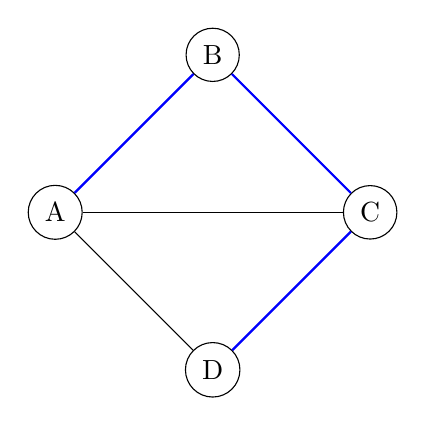
\begin{tikzpicture}
    % Define the vertices
    \node[draw, circle] (A) at (0, 0) {A};
    \node[draw, circle] (B) at (2, 2) {B};
    \node[draw, circle] (C) at (4, 0) {C};
    \node[draw, circle] (D) at (2, -2) {D};
    
    % Define the edges
    \draw (A) -- (B);
    \draw (B) -- (C);
    \draw (C) -- (D);
    \draw (A) -- (C);
    \draw (A) -- (D);
    
    % Highlight the Hamiltonian Path A-B-C-D
    \draw[blue, thick] (A) -- (B);
    \draw[blue, thick] (B) -- (C);
    \draw[blue, thick] (C) -- (D);
\end{tikzpicture}
\end{center}

For the directed graphs below, the graph on the left has a Hamiltonian Path from A to D, while the graph on the right does not have a Hamiltonian Path from A to D.

\begin{center}
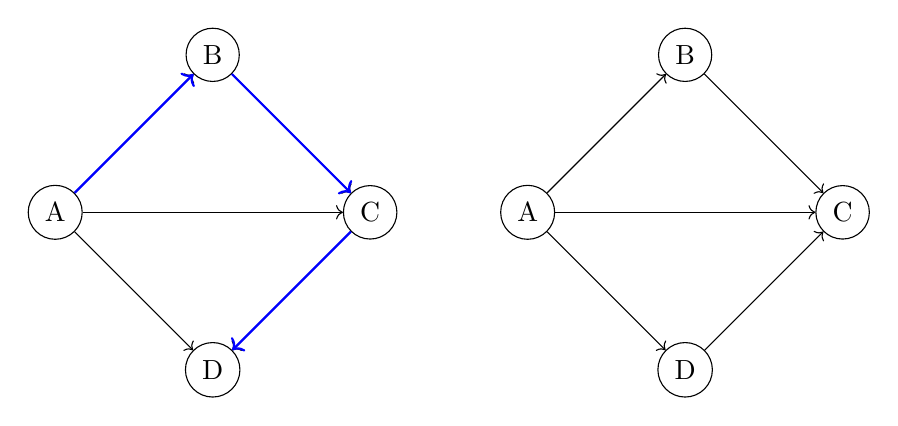
\begin{tikzpicture}
    % First graph with Hamiltonian Path
    \node[draw, circle] (A1) at (0, 0) {A};
    \node[draw, circle] (B1) at (2, 2) {B};
    \node[draw, circle] (C1) at (4, 0) {C};
    \node[draw, circle] (D1) at (2, -2) {D};
    
    \draw[->] (A1) -- (B1);
    \draw[->] (B1) -- (C1);
    \draw[->] (C1) -- (D1);
    \draw[->] (A1) -- (C1);
    \draw[->] (A1) -- (D1);
    
    \draw[blue, thick, ->] (A1) -- (B1);
    \draw[blue, thick, ->] (B1) -- (C1);
    \draw[blue, thick, ->] (C1) -- (D1);

    % Second graph without Hamiltonian Path
    \node[draw, circle] (A2) at (6, 0) {A};
    \node[draw, circle] (B2) at (8, 2) {B};
    \node[draw, circle] (C2) at (10, 0) {C};
    \node[draw, circle] (D2) at (8, -2) {D};
    
    \draw[->] (A2) -- (B2);
    \draw[->] (B2) -- (C2);
    \draw[->] (D2) -- (C2);
    \draw[->] (A2) -- (C2);
    \draw[->] (A2) -- (D2);

\end{tikzpicture}
\end{center}

We refer to the undirected version of this problem as \textbf{UHP} and the directed version as \textbf{DHP}.

\begin{questions}

    \question[3] Give a reduction from UHP to DHP.

      \begin{soln}
      Given an undirected graph $G = (V, E)$, we can construct a directed graph $G' = (V', E')$ as follows:
      \begin{itemize}
          \item For each vertex $v \in V$, create a vertex $v' \in V'$.
          \item For each edge $(u, v) \in E$, create two directed edges $(u', v')$ and $(v', u')$ in $E'$.
          \item Or more concisely, we have to make the edge $u \rightarrow v$ and $v \rightarrow u$ for all edges in the 
          UHP, into DHP
      \end{itemize}
      Since every edge in the original graph becomes two directed edges 
      (one in each direction), all the paths that existed in the undirected 
      graph still exist in the directed one. In particular, 
      any Hamiltonian Path from $s$ to $t$ in the undirected graph corresponds 
      exactly to a Hamiltonian Path from $s$ to $t$ in the directed graph.

      This implies that solving the problem in the directed graph will also 
      solve the problem in the undirected graph.
      \end{soln}

    \ifsolutions\input{q1a-sol.tex}\fi

    \question[4] Prove the correctness of your reduction from UHP to DHP. That is, prove that the answer to your reduced DHP instance is YES if and only if the answer to UHP is YES. 

      \begin{soln}
            To prove the correctness of the reduction, we want to show that;
            \[ 
            \text{If the original UHP instance is YES} 
            \iff 
            \text{the reduced DHP instance is YES} 
            \]
            \begin{proof}

                  \textbf{$\Rightarrow$ Direction: If UHP instance is YES}

                  We assume first that the original UHP instance is YES.
                  That implies that there exists a Hamiltonian Path from 
                  $s$ to $t$ in $G$ that visits every vertex exactly once.
                  Since $G\prime$ contains all vertices of $G$ and for every undirected
                  edge from $(u, v) \in G$ we have both $(u, v) \wedge (v, u) \in G\prime$,
                  we can also follow the exact same path as in $G$ in $G\prime$.
                  Therefore, we can find a Hamiltonian Path from $s$ to $t$ in $G\prime$ 
                  that visits every vertex exactly once.

                  \textbf{$\Leftarrow$ Direction: If DHP instance is YES}

                  Now we assume that the reduced DHP instance is YES.
                  That means that there exists a directed Hamiltonian Path.
                  Since every edge in $G\prime$ comes from a corresponding undirected
                  edge in $G$, we can follow the same path in $G$ as in $G\prime$.
                  Therefore, we can find a Hamiltonian Path from $s$ to $t$ in $G$ 
                  that visits every vertex exactly once.
            \end{proof}
      \end{soln}


    \ifsolutions\input{q1b-sol.tex}\fi

    \question[7] Give a reduction from DHP to UHP. You \textbf{do not} need to prove the correctness of this reduction, but you should clearly explain the key components of your reduction and why they are there.

    \begin{soln}
      To reduce from DHP to UHP, we first have to understand that directed graphs
      flows a certain way, that is, the edges are directed. 
      In order to convert this ``directional-ness'' into an undirected graph, we can introduce
      two new vertices for every $v \in V$ such that the 
      new vertices are $v_{in}$ and $v_{out}$. So then the edges will look something like this
      \[
      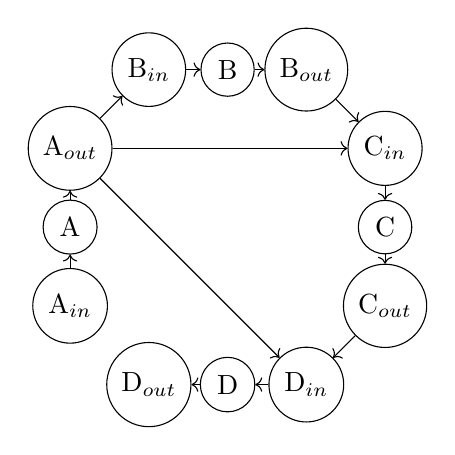
\begin{tikzpicture}
            \node[draw, circle] (A) at (0, 0) {A};
            \node[draw, circle] (B) at (2, 2) {B};
            \node[draw, circle] (C) at (4, 0) {C};
            \node[draw, circle] (D) at (2, -2) {D};


            \node[draw, circle] (A_in) at (0, -1) {A$_{in}$};
            \draw[->] (A_in) -- (A);
            \node[draw, circle] (A_out) at (0, 1) {A$_{out}$};
            \draw[->] (A) -- (A_out);

            \node[draw, circle] (B_in) at (1, 2) {B$_{in}$};
            \draw[->] (B_in) -- (B);
            \node[draw, circle] (B_out) at (3, 2) {B$_{out}$};
            \draw[->] (B) -- (B_out);

            \node[draw, circle] (C_in) at (4, 1) {C$_{in}$};
            \draw[->] (C_in) -- (C);
            \node[draw, circle] (C_out) at (4, -1) {C$_{out}$};
            \draw[->] (C) -- (C_out);

            \node[draw, circle] (D_in) at (3, -2) {D$_{in}$};
            \draw[->] (D_in) -- (D);
            \node[draw, circle] (D_out) at (1, -2) {D$_{out}$};
            \draw[->] (D) -- (D_out);
            
            % Define the edges
            \draw[->] (A_out) -- (B_in);
            \draw[->] (B_out) -- (C_in);
            \draw[->] (C_out) -- (D_in);
            \draw[->] (A_out) -- (C_in);
            \draw[->] (A_out) -- (D_in);
      \end{tikzpicture}
      \]
      This gadget will allow us to convert the directed edges 
      into undirected edges, by forcing it through a certain path, in this case, 
      in the direction of $v_{in} \rightarrow v \rightarrow v_{out}$.
      So, for every directed edge $(u, v) \in E$, add the undirected edge 
      $u_{out} - v_{in}$ to the undirected graph.
    \end{soln}
    \ifsolutions\input{q1c-sol.tex}\fi


\end{questions}

%===============================
\section{Strategically Placed Krispy Kremes}

This SPKK problem is also in Tutorial 6. UBC Rec student leaders are planning their next fundraiser, and are seeking your help in identifying strategic locations to set up their stands of Krispy Kremes. They have a map showing $n$ locations of buildings and outdoor spots on campus. Their $k$ stands need to be set up in the outdoor spots. They want you to select $k$ spots such that the maximum distance from any of the $n$ locations to a stand is as small as possible.

An instance of the Strategically Placed Krispy Kremes decision problem (SPKK) has a set $V$ of size $n$, a subset $S$ of $V$, an integer $k$, $1\le k \le |S|$,  and a symmetric matrix $d[1..n][1..n]$, plus an additional nonnegative integer $b$. The problem is to determine if there is a subset $S' \subseteq S$ of size $k$, such that

\[
\max_{v \in V} \min_{s \in S'} \{ d[v][s] \;|\; s \in S' \} \le b.
\]

\begin{questions}
\question[8]
Provide a reduction from the Dominating Set problem to SPKK.
Briefly justify why the reduction is polynomial-time (one sentence is sufficient). Carefully explain why your reduction is correct (two paragraphs is sufficient).

\begin{soln}
      In the Dominating Set problem, we are given a graph $G = (V, E)$ 
      and an integer $k$, and we want to determine if there 
      is a subset $D \subseteq V$ of size $k$ such that every vertex 
      in $V$ is either in $D$ or adjacent to a vertex in $D$.

      So connecting back to our SPKK problem, we can see that 
      we have a set $V$ of locations, a subset $S \subseteq V$, where we 
      can put our stands, and a distance matrix $d$. The goal is to choose $k$
      spots from $S$ such that every location $V$ is ``close'' 
      (within distance $b$) to at least one of the stands. 
      There is a technique we can use, and that is to convert the graph
      structure into the distance matrix so that the property if Dominating Set
      perfectly matches our condition that every vertex is within a distance $b$
      of a chosen stand.
      
      $\textbf{Constructing our reduction: }$
      \begin{enumerate}
            \item Instance Transformation:
            \begin{itemize}
                  \item Let the set $V$ in the Dominating Set instance be both
                  the set of vertices and the $S$ where stand can be placed, (i.e. $S = V$).
                  \item Then, we can define the matrix $d$ as follows:
                  \begin{itemize}
                        \item $d[u][v] = 0 \Leftrightarrow u = v$ (the distance from a vertex to itself is 0)
                        \item $d[u][v] = 1 \Leftrightarrow (u, v) \in E$ (the distance from a vertex to its neighbour is 1)
                        \item $d[u][v] = 2 \Leftrightarrow (u, v) \notin E$ (the distance from a vertex to its non-neighbour is 2)
                  \end{itemize}
                  \item Then we set the bound $b = 1$, because we want to ensure that 
                  every vertex is either in $D$ or adjacent to a vertex in $D$, 
                  (even if it is inefficient, at least it is better than non-polynomial time.)
            \end{itemize}
            \item Correctness of the reduction:
            
            ``If the graph has dominating set of size $k$''
            Assume that we indeed have a dominating set $D \subseteq V$ with 
            $|D| = k$. Then that means, for every vertex $v \in V$, 
            either $v$ is in $D$ (so that $d[v][s] = 0$) or 
            $v$ is adjacent to a vertex in $D$ (so that $d[v][s] = 1$).
            In either case, the maximum over all vertices of these minimum distances
            is at most 1. 

            Therefore, it must be true that, the maximum distance from any vertex
            to a stand is at most 1, which is less than or equal to $b$. Ultimately,
            implying that the SPPK instance with bound $b = 1$ is a YES instance.

            ``If the graph does not have a dominating set of size $k$''
            Assume that we have a subset $S\prime \subseteq S$ with $|S\prime| = k$.
            Such assumptions implies that every vertex $v \in V$ is at most 
            distance 1 from some $s \in S\prime$. This means for each $v$, either
            $v \in S\prime$ giving $d[v][v] = 0$ or there is some $s \in S\prime$
            $d[v][s] = 1$, which implies that $v$ and $s$ are neighbours.
            Therefore, every vertex is either in $S\prime$ or adjacent to a vertex
            in $S\prime$, so $S\prime$ is a dominating set of size $k$.
      \end{enumerate}
      $\textbf{Polynomial-Time Reduction Justification: }$
      The reduction is polynomial-time because the construction of the distance matrix
      $d$ takes $O(n^2)$ time, where $n$ is the number of vertices in the graph $G$.
      The construction of the distance matrix is a simple operation of
      iterating through the vertices and edges of the graph, and filling in the
      distance matrix accordingly. The other steps of the reduction, such as
      defining the set $S$ and the bound $b$, are also simple operations that
      can be done in polynomial time. Therefore, the overall reduction is polynomial-time.
\end{soln}
 
  \ifsolutions\input{q1a-sol.tex}\fi
  \end{questions}


\section{Very Special Problems}

In this question, we consider special cases of NP-complete problems. Formally, we say that Problem B is a \textbf{special case} of Problem A if every instance of Problem B can be viewed as an instance of Problem A. We've seen examples of this in class: for example, 3-SAT is a special case of SAT (where every clause has length 3). Minimum spanning tree is a special case of Steiner Tree, in which the set of vertices we need to connect includes all the vertices in $V$.

\begin{questions}

\question[4] Consider the \textbf{Bounded-Leaf Spanning Tree Problem (BLST)}: given a graph $G = (V,E)$ and an integer $k$, does $G$ have a spanning tree with no more than $k$ leaves?

Give an NP-complete problem that is a special case of BLST, and justify why this problem is a special case.

\ifsolutions\input{q3a-sol.tex}\fi

\question[3] You showed in the previous question that there is an NP-complete problem that is a special case of BLST, and it is not difficult to show that BLST is in NP (though we are not asking you to do this). Does this imply that BLST is NP-complete? Justify your answer.

\ifsolutions\input{q3b-sol.tex}\fi

\question[4] Give an example of a polytime-solvable problem you have seen in this class that is a special case of an NP-complete problem. Justify your answer.

\ifsolutions\input{q3c-sol.tex}\fi

\end{questions}

\end{document}